\documentclass[10pt]{article}


\usepackage{amsmath}
\usepackage{amsthm}
\usepackage{amssymb}
\usepackage{fullpage}
\usepackage{cite}
\usepackage{hyperref}
\usepackage{ifthen}
\usepackage{subcaption}
\usepackage{graphicx}
\usepackage[linesnumbered, nofillcomment,noend]{algorithm2e}
\usepackage{stackrel}

\usepackage{mathtools}

\DeclarePairedDelimiter\ceil{\lceil}{\rceil}
\DeclarePairedDelimiter\floor{\lfloor}{\rfloor}


\title{}
\author{Logan Withers}
\date{}



\begin{document}

    \begin{flalign*}
       \text{Let }  m & = \text{base of the counter} & \\
                    l & = \ceil{\log m} + 2,                  \text{ number of bits needed to represent each digit plus 2 for MSR and MSD} & \\
                c_{0} & = \text{starting value of counter}  \\
                c_{f} & = m^{\ceil*{\log_m{c_{0}} }} - 1,     \text{ final value of the counter}                     \\
           c_{\Delta} & = c_f - c_0,                          \text{ number of times the counter increments}         \\
                    d & = \ceil*{\log_m({c_0})},              \text{ number of digits in each value of the counter } \\
                  d_r & = \ceil*{\frac{d}{3}},                \text{ number of digit regions}                        \\
    \mathcal{H}_{d_r} & = 3 \cdot (l + 30),                   \text{ height of a digit region }                      \\
                    N & = c_{\Delta} \cdot \mathcal{H}_{d_r}, \text{ height of entire rectangle }                    \\
                    K & = 2 \cdot d,                          \text{ width of }
    \end{flalign*}


    \begin{figure}
        \centering

        \begin{subfigure}[t]{0.23\textwidth}
            \centering
            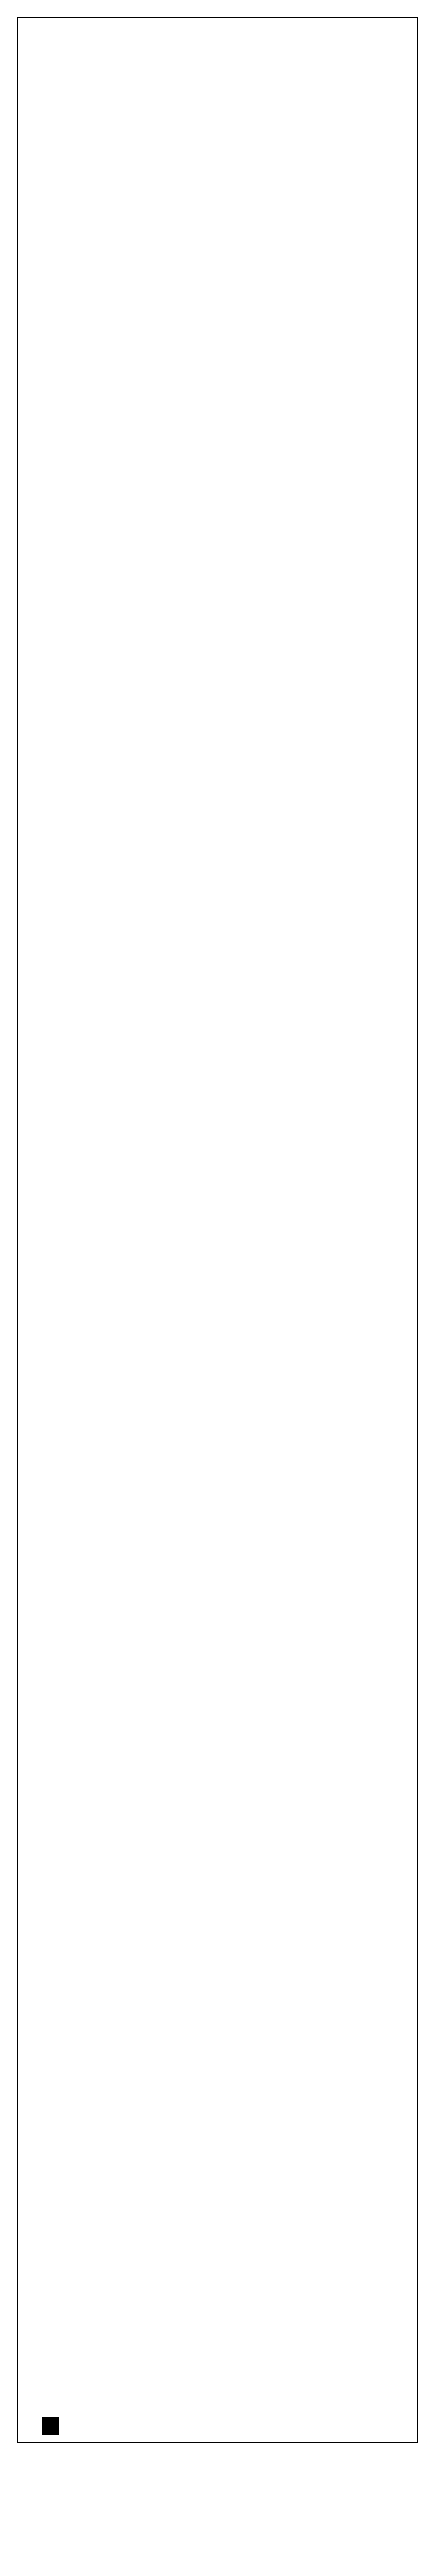
\includegraphics[width=.85in]{mid_level_timeline_phase_1}
            \caption{\label{fig:mid_level_timeline_phase_1} A subassembly of $\alpha$ and a window $w$ induced by a translation of the $y$-axis.}
        \end{subfigure}%
    %     ~
    %     \begin{subfigure}[t]{0.23\textwidth}
    %         \centering
    %         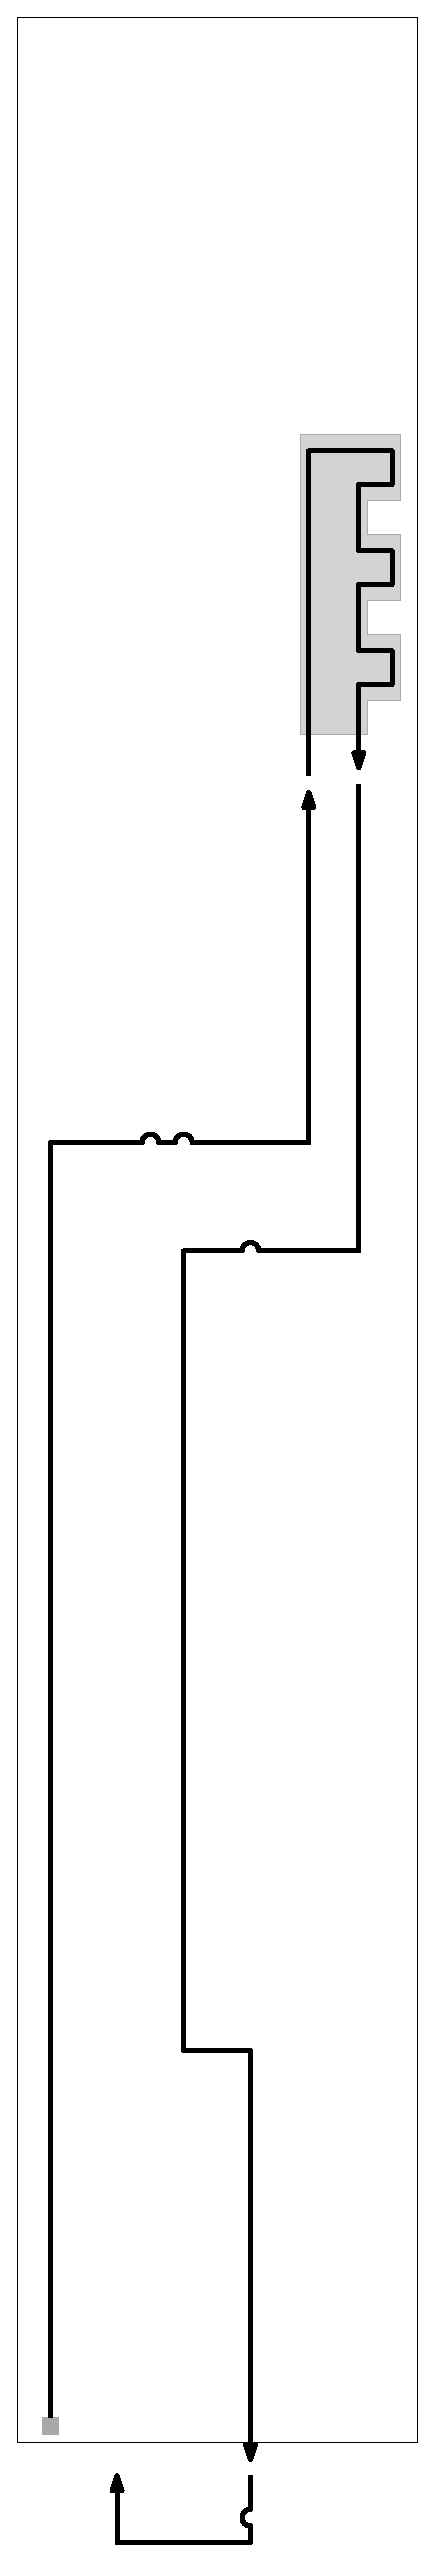
\includegraphics[width=.85in]{mid_level_timeline_phase_2.eps}
    %         \caption{\label{fig:mid_level_timeline_phase_2} A portion of the simple path $s$ through $G^b_{\alpha}$.}
    %     \end{subfigure}%
    %    ~
    %     \begin{subfigure}[t]{0.23\textwidth}
    %         \centering
    %         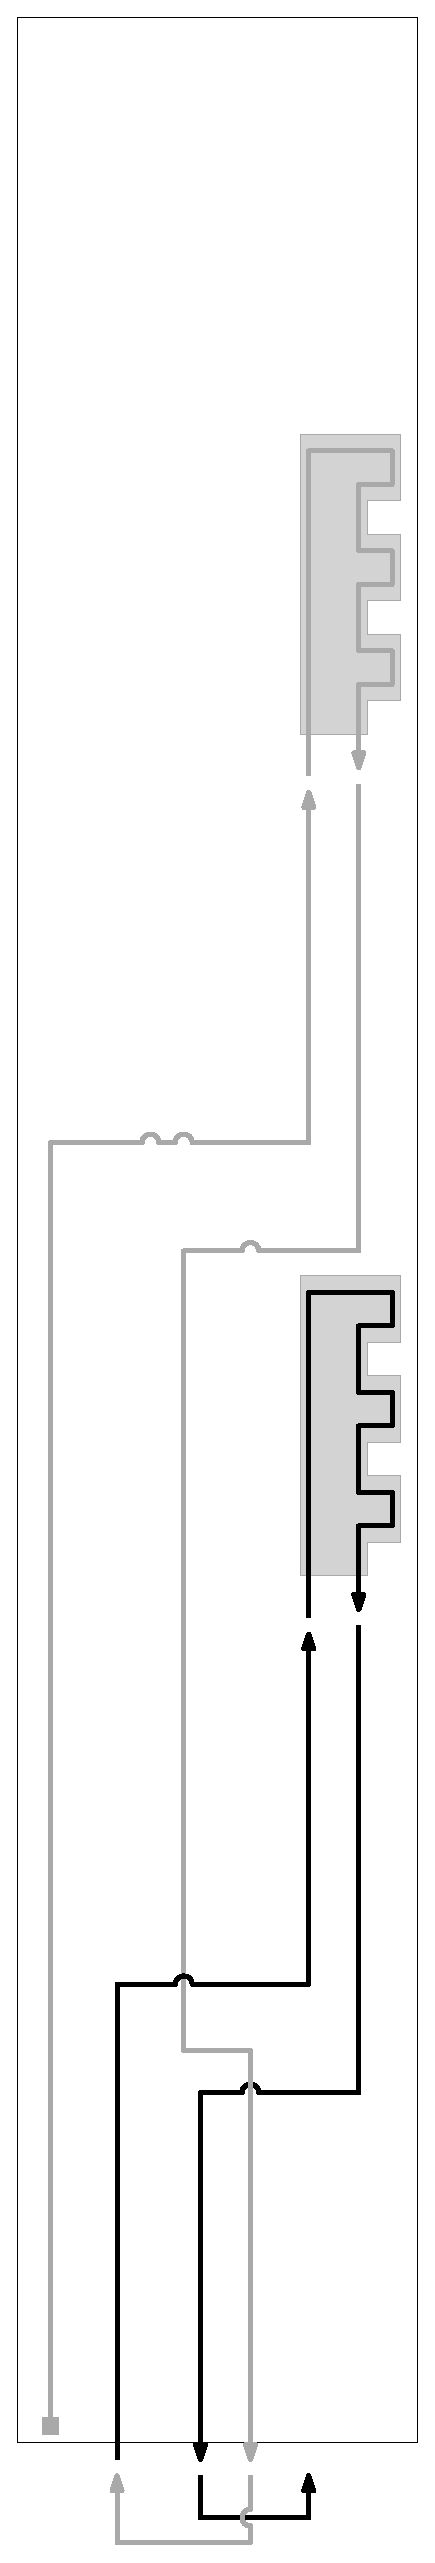
\includegraphics[width=.85in]{mid_level_timeline_phase_3.eps}
    %         \caption{\label{fig:mid_level_timeline_phase_3} The glue window movie $M_{\vec{\alpha},w}$ }
    %     \end{subfigure}%
    %     ~
    %     \begin{subfigure}[t]{0.23\textwidth}
    %         \centering
    %         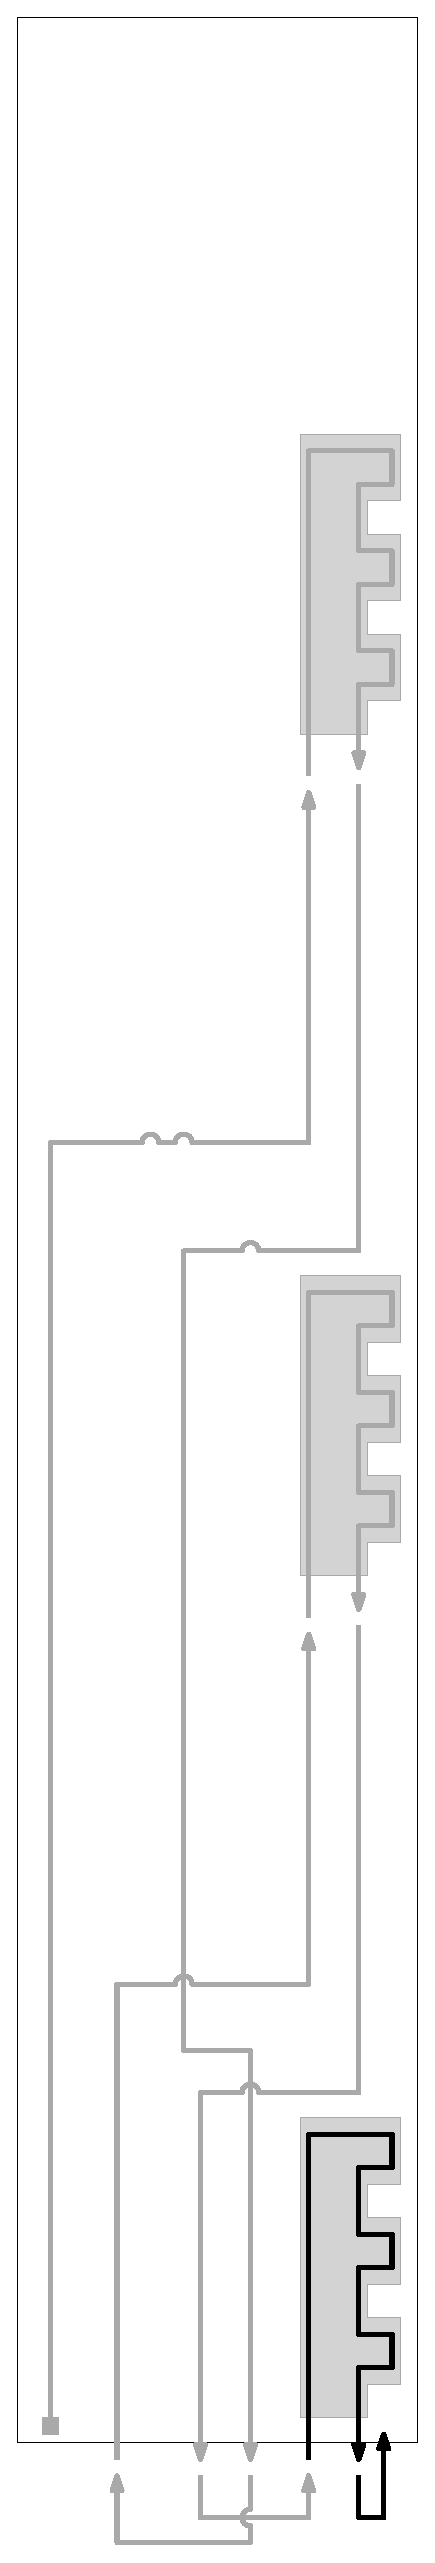
\includegraphics[width=.85in]{mid_level_timeline_phase_4.eps}
    %         \caption{\label{fig:mid_level_timeline_phase_4} The restricted glue window submovie $M_{\vec{\alpha},w} \upharpoonright s$ }
    %     \end{subfigure}
        \caption{\label{fig:mid_level_timeline_overview} An assembly, a simple path and the various types of glue window movies. }
    \end{figure}

    % \subsubsection*{Counter Writers}



    % \subsubsection*{Warp Units}

    %     \noindent\texttt{Pre\_First\_Warp}

    %     \noindent\texttt{First\_Warp}

    %     \noindent\texttt{Warp\_Bridge}

    %     \noindent\texttt{Second\_Warp}

    %     \noindent\texttt{Post\_Warp}



    % \subsubsection*{Digit Top}

    %     \noindent\texttt{DigitTop}

    %     \noindent\texttt{DigitTop\_Digit1}

    %     \noindent\texttt{DigitTop\_Digit2}

    %     \noindent\texttt{DigitTop\_Digit3}



    % \subsubsection*{ReturnDigitNReadDigitN+1}

    %     \noindent\texttt{ReturnDigit1\_ReadDigit2}

    %     \noindent\texttt{ReturnDigit2\_ReadDigit3}

    %     \noindent\texttt{ReturnDigit3\_ReadDigit1}


    % \subsubsection*{ReturnDigitNReadNextRow}

        % \noindent\texttt{ReturnDigit1\_ReadNextRow}

        % \noindent\texttt{ReturnDigit2\_ReadNextRow}

        % \noindent\texttt{ReturnDigit3\_ReadNextRow}

\end{document}